\chapter{Theoretical framework}
\label{ch:theory}

\section{Introduction}
The behaviour of fundamental particles and forces are described by the Standard Model (SM) of
particle physics.
For a long time validation of the SM relied upon the discovery of a scalar Higgs boson, which was
observed in 2012 \cms and \atlas collaborations.
This final piece of the picture has made the SM a remarkably robust theory with no predictions
deviating from experimental observations.
Indeed, the fine structure constant, $\alpha$, which characterizes the coupling strength of
electromagnetic interactions is one of the most accurately predicted physical values.
The value of $\alpha^{-1}$ is measured to be:
\begin{equation}
  \alpha^{-1} = 137.035 999 074 (44),
\end{equation}
with a relative uncertainty of 0.32 parts per billion~\cite{PDG2012}, while the current best theoretical
prediction, which accounts for up to tenth order Feynman diagrams, is:
\begin{equation}
  \alpha^{-1} = 137.035 999 073 (35),
\end{equation}
to an accuracy of 0.25 parts per billion~\cite{Aoyama:2012wj}.
The agreement of these values makes the theory of Quantum Electrodynamics, which describes
interactions of photons and charged particles in the SM, one of the most accurate theories yet
constructed.

%Despite countless measurements being in agreement with SM theoretical predictions, it is well known
Despite its countless successes,
there are many experimental and theoretical arguments indicating that the SM is an incomplete
picture of particle physics.
Many theoretical problems arise from the idea of naturalness, that is that...

%Experimental observations that are it is well known that the SM is incomplete; arguments for this
%come from both the experimental and theoretical
%leaves some experimentally observed phenomena unexplained.
Experimentally, there are observed phenomena which are left unexplained by the SM.
Neutrinos are treated as massless in the SM, but they are seen to oscillate in flavour space
indicating that they must, in fact, have mass.
Flat rotation curves of galaxies and gravitational lensing indicate the existence of Dark Matter,
which is entriely unaccounted for by the SM.
%Shortcomings include the
% credence
%For example the SM does not explain: gravity, dark matter, dark energy, and neutrino masses.

Another problem is that the SM cannot reconcile the matter-antimatter asymmetry observable in the
Universe today.
The hypothesized process which caused this asymmetry is known as baryogenesis.
%Baryogenesis is the term for a hypothesized process which resulted in the matter-dominated nature of
%the Universe.
Whatever this process may be, it must satisfy:
\begin{itemize}
  \item at least one baryon number (B) violating process,
  \item Charge and Charge-Parity (CP) violation,
  \item interactions out of thermal equilibrium.
\end{itemize}
These are the Sakharov conditions~\cite{1991SvPhU..34..392S}, and outline the minimum requirements
of baryogenesis.
The first of these criteria is an obvious one: at the time of the Big Bang $B=0$, whereas today
$B\gg0$; hence $B$ must not be conserved in some process.
If a process conserves charge then
\begin{equation}
  \Gamma(X\to Y+B)=\Gamma(\bar X \to \bar Y+\bar B),
\end{equation}
so $B$ will be conserved over time.
However, this condition is insufficient.
Consider a process $X\to q_Lq_L$ which has a CP-conjugate process $\bar X\to \bar q_R\bar q_R$;
then
\begin{equation}
  \Gamma(X\to q_Lq_L) + \Gamma(X\to q_Rq_R)
  =
  \Gamma(\bar X\to \bar q_R\bar q_R) + \Gamma(\bar X\to \bar q_L\bar q_L)
\end{equation}
would still result in $B$ conservation even if C is violated.
Thus, the process must be CP violating.
The final criteria ensures that baryogenesis occurs at a higher rate than anti-baryogenesis.
%Clearly the process must result in the violation of baryon number, and it must happen out of
%thermal equilibrium otherwise the process would occur equally as often in each direction.
%The third condition, CP violation (CPV) means that
%$\Gamma(A+B\to C)\neq\Gamma(\bar A + \bar B \to \bar C)$, so the annihilation of the products of
%the interaction cannot washout the asymmetry.

The flavour sector is the only source of CPV in the SM, but comes up short by around 10 orders of
magnitude when explaining the matter dominated nature of the Universe~\cite{Cline:2006ts,Huet:1994jb}.
%There is therefore a powerful reason to believe that NP enters the flavour sector.
The following chapter will elucidate as to how the flavour sector is the only source of CPV in the
SM.




\section{The Standard Model}
The current formulation of the SM of particle physics was concocted in the 1970s, when the Higgs
mechanism was incorporated into Glashow's electroweak theory by Salam and Weinberg.
The theory prescribes a treatment
as to how fundamental particles interact via three of the four
fundamental forces, namely: the strong, weak and electromagnetic forces.

%Mathematically, the SM is a locally gauge invariant quantum field theory, where excitations of
%various fields manifest themselves as particles.
%There is a global Poincare symmetry as required by special relativity; and a local
%$SU(3)\times SU(2)\times U(1)$ symmetry which encapsulates the SM Lagrangian:
%\begin{equation}
  %\Lag{SM} = \Lag{EW} + \Lag{Strong} + \Lag{Higgs}.
%\end{equation}
%Where the components describe the electroweak, strong and Higgs interactions.
%Each generator of this local gauge group is associated with a gauge boson which mediates
%interactions between other bosons and fermions.

Mathematically, the SM is a locally gauge invariant quantum field theory.
It inhabits a space-time with a global Poincar\'e symmetry that obeys a local
$SU(3)\times SU(2)\times U(1)$ symmetry.
Each generator in this group corresponds to a gauge-boson; so the strong force ($SU(3)$ group) has
eight gluons that mediate the interaction, and the electroweak force ($SU(2)\times U(1)$ group) has
$3+1$ gauge bosons, which are the weak gauge bosons ($Z$, $W^\pm$) and the photon ($\gamma$).
These are all vector fields.
Fermions are described by spinor fields, $\psi$, which obey the Dirac equation:
\begin{equation}
  (i\hbar\gamma^\mu\partial_\mu - mc)\psi = 0.
  \label{th:eq:dirac}
\end{equation}
The fermions of the SM constitute six leptons (electron, electron neutrino, muon, muon neutrino,
tau and tau neutrino) and six quarks (up, down, charm, strange, top and bottom), which are
organized into pairs forming three generations.
For each fermion there is a corresponding antiparticle with the same mass and opposite charge ---
charge being the conserved quantity resulting from the global gauge symmetry (by Noether's
theorem).
There is also a single scalar field in the SM, that of the Higgs boson.
%The only additional particle is the scalar Higgs boson.

The SM Lagrangian can be expressed as a sum of components:
\begin{equation}
  \Lag{SM} = \Lag{Strong} + \Lag{V} + \Lag{\ell} + \Lag{\it q} + \Lag{Higgs} + \Lag{Yuk}.
  \label{eq:th:lag}
\end{equation}
The first three terms describe: interactions of the strong force between colour carrying particles,
weak vector boson self-interactions, and the electroweak behavior of leptons.
The remaining terms describe the electroweak behavior of quarks, the Higgs interaction and Yukawa
couplings, respectively.
These latter terms are of fundamental importance as to how the flavour changing currents and CPV
occur in the SM, and will be be discussed in detail.
%the SM.
%Each of these shall be discussed in turn.

The structure of CP and flavour violation emerges as a direct consequence of the Higgs mechanism
breaking the local electroweak symmetry.
The Lagrangian of the scalar Higgs field is:
\begin{align}
  \Lag{Higgs}
  &= \left(D_\mu\Phi\right)^\dagger\left(D^\mu\Phi\right) - V(\Phi) \\
  &= \left(D_\mu\Phi\right)^\dagger\left(D^\mu\Phi\right) - \mu^2\left(\Phi^\dagger\Phi\right) +
  \lambda\left(\Phi^\dagger\Phi\right),
  \label{eq:th:laghiggs1}
\end{align}
where $\mu$ and $\lambda$ are constants, $D_\mu$ is the covariant derivative, and $\Phi$ is the
Higgs doublet, defined by:
\begin{equation}
  \Phi = \frac{1}{\sqrt{2}}
  \begin{pmatrix}
    \phi_1 + i\phi_2 \\
    \phi_3 + i\phi_4 \\
  \end{pmatrix}.
  \label{eq:th:phi}
\end{equation}
Taking $\mu^2<0$ and $\lambda>0$ moves the minimum of the potential $V(\Phi)$ away from zero to a distance $v$:
\begin{equation}
  v = \sqrt{\frac{\mu^2}{\lambda}}.
\end{equation}
At this point the Higgs field gets a vacuum expectation value (VEV)
%$\braket{\phi} = \tfrac{1}{\sqrt{2}}v$.
of $\langle\phi\rangle = \tfrac{1}{\sqrt{2}}v$.
The direction of the VEV from the origin is arbitrary, but the choice of:
\begin{align}
  \bra{0}\phi_1\ket{0} =
  \bra{0}\phi_2\ket{0} =
  \bra{0}\phi_4\ket{0} = 0  &&
  \bra{0}\phi_3\ket{0} = v,
\end{align}
is convenient, and changes Eq.~\ref{eq:th:phi} to:
\begin{equation}
  \Phi = \frac{1}{\sqrt{2}}
  \begin{pmatrix}
    \eta_1 + i\eta_2 \\
    v + i\eta_4 \\
  \end{pmatrix}.
  \label{eq:th:eta}
\end{equation}
Here, $\eta_1$, $\eta_2$ and $\eta_4$, are Goldstone bosons which, by choosing an appropriate
gauge, become the longitudinal components of the weak bosons.
This choice of gauge simplifies $\Phi$ to:
\begin{equation}
  \Phi =
  \begin{pmatrix} 0 \\ v+H
  \end{pmatrix},
  \label{eq:th:phi2}
\end{equation}
where $H$ is the physical Higgs boson.
%Using this in Eq.~\ref{eq:th:laghiggs1} gives:
Inserting Eq.~\ref{eq:th:phi2} into Eq.~\ref{eq:th:laghiggs1} gives:
%\begin{multline}
  %\Lag{Higgs} =
  %\frac12\left(\partial_\mu H\right)\left(\partial^\mu H\right)
  %+\frac14g^2\left(v^2 + 2vH + H^2\right)W_\mu^+W^{-\mu}  \\
  %+\frac18\left(g^2 + g^{\prime2}\right)\left(v^2 + 2vH + H^2\right)Z_\mu Z^\mu
  %+ \mu^2H^2 + \frac14\lambda\left(H^4+4vH^3\right) + \cdots,
  %\label{eq:th:laghiggs2}
%\end{multline}
\begin{equation}
  \Lag{Higgs} =
  \frac12\left(\partial_\mu H\right)\left(\partial^\mu H\right)
  +\mu^2H^2
  +\left(m_W^2W_\mu^+W^{-\mu} + \frac{m_Z^2}{2}Z_\mu Z^\mu\right)
  \cdot
  \left(1 + \frac{H}{v}\right)^2
  \label{eq:th:laghiggs2}
\end{equation}
where $g$ and $g^\prime$ are coupling constants and other terms are three- and four-point
interactions of the Higgs with itself and weak gauge bosons.
Thus, the $U(1)$ local gauge symmetry is broken, weak gauge boson acquire a mass while photons remain
massless; as is consistent with observations.


%It is not possible to directly insert mass terms for fermions, because the required terms
%($m(\bar\psi_L\psi_R+\bar\psi_R\psi_L$) are not allowed \bam{ELABORATE}.
All fermions (except neutrinos) also get a mass after the spontaneous symmetry breaking (SSB) of
the $U(1)$ symmetry.
The Dirac mass term for a chiral field should be of the form:
\begin{equation}
  \Lag{mass} = -m_\psi\left(\bar\psi_R\psi_L + \bar\psi_L\psi_R\right),
\end{equation}
but the left- and right-handed fields have different $U(1)$ charges %Y hypercharge
and so transform differently under local gauge transformations and so cannot be added to \Lag{SM}.
However, masses can be generated through the Yukawa couplings (\Lag{Yuk} in \Eq{eq:th:lag}), which
describe integrations between all fermionic fields and the Higgs doublet, and can be written:
\begin{equation}
  \Lag{Yuk} = \sum_{\substack{\ell=\\e,\mu,\tau}}\left(\Lag{Yuk}^\ell\right) + \Lag{Yuk}^q,
  \label{eq:th:yukking}
\end{equation}
where $\ell$ and $q$ denote the lepton and quark sectors respectively.
First considering the lepton term, after SSB:
\begin{align}
  \Lag{Yuk}^\ell
  &= - g_\ell\left(\bar\chi_L\Phi \ell_R + \bar \ell_R\Phi^\dagger\chi_L\right) \\
  &= - \frac{g_\ell v}{\sqrt{2}}\left(\bar\ell_L\ell_R + \bar\ell_R\ell_L\right)\cdot
  \left(1 + \frac{H}{v}\right)
     %- \frac{g_\ell}{\sqrt{2}}H\left(\bar\ell_L\ell_R + \bar\ell_R\ell_L\right),
\end{align}
where $g_\ell$ is a coupling constant, and
\begin{align}
  \chi_L = \begin{pmatrix}\nu_L \\ \ell_L \end{pmatrix}.
\end{align}
Thus the leptons get a mass of $m_\ell = \tfrac{1}{\sqrt{2}}g_\ell v$, and interact with the Higgs
field.

The story for $\Lag{Yuk}^q$ is a bit more involved.
Before SSB:
\begin{align}
  \Lag{Yuk}^q &= - y_{ij}^u\bar Q_L^i\Phi u_R^j
  - y_{ij}^d\bar Q_L^i\tilde\Phi d_R^j + \mathrm{h.c.},
  \label{eq:th:lagyukq}
\end{align}
where there is an implicit sum over all generations $i$ and $j$, $y^{u,d}$ is a $3\times3$ matrix
characterizing the Yukawa couplings between quark generations,
\begin{align}
  \tilde\Phi_i &= \varepsilon_{ij}\Phi_j,
    \qquad \mathrm{and} \quad Q_L = \begin{pmatrix}u_L \\ d_L \end{pmatrix}.
\end{align}
After SSB, and the Higgs acquires a VEV, \Eq{eq:th:lagyukq} becomes:
\begin{equation}
  \Lag{Yuk}^q =
  - \frac{v}{\sqrt{2}}
  \left(
  y_{ij}^u\bar u_L^iu_{R,j}
  + y_{ij}^d\bar d_L^id_{R,j},
  + \mathrm{h.c.}
  \right)
  \cdot
  \left(1 + \frac{H}{v}\right),
  \label{eq:th:lagyuk2}
\end{equation}
where the mass of the quarks is $m_q = \frac{v}{\sqrt{2}}y_{ij}^q$.
However, it is more convenient to change a basis in which the matrix $m^q$ is diagonal such that
$m_{ij}^\mathrm{diag} = V_{Lik}m_{kl}(V_R^\dagger)_{lj}$.
This is exactly equivalent to transforming the chiral quark fields for up- and down-type quarks
accordingly:
\begin{align}
  q_L^\alpha = \left(V_L^q\right)_{\alpha i}q_L &&
  q_R^\alpha = \left(V_R^q\right)_{\alpha i}q_R,
\end{align}
where the index of the original basis is identified with $i$ and the mass basis uses $\alpha$.

The rotations of the basis of the chiral quark fields leave much of \Lag{SM} unchanged since
$V_{qL}^\dagger V_{qL} = V_{qR}^\dagger V_{qR} = \mathbb{1}$.
However, this is not the case in the charged current (CC) part of \Lag{\it q}; which transforms as:
\begin{align}
  \Lag{\it q}^\mathrm{CC}
  &= \frac{g}{2}i\gamma^\mu
  \left[\bar u_Ld_LW^+_\mu + \bar d_Lu_LW^-_\mu
  \right]  \\
  &= \frac{g}{2}i\gamma^\mu
  \left[
    \bar u_L\left(V_{uL}V_{dL}^\dagger\right)d_LW^+_\mu +
    \bar d_L\left(V_{dL}V_{uL}^\dagger\right)u_LW^-_\mu
  \right]  \\
  &= \frac{g}{2}i\gamma^\mu
  \left[
    V\bar u_Ld_LW^+_\mu +
    V^\dagger\bar d_Lu_LW^-_\mu
  \right].
\end{align}
The matrix $V$ is defined is known as the Cabibbo-Kobayashi-Maskawa (CKM) matrix
and parameterizes the couplings between up- and down-type quarks in charged weak currents.






\section{The CKM matrix and Unitarity Triangle}
\label{sec:ckm}

The CKM matrix is defined as:
\begin{equation}
  V = \left(V_{uL}V_{dL}^\dagger\right) =
  \begin{pmatrix}
    \V{ud} & \V{us} & \V{ub} \\
    \V{cd} & \V{cs} & \V{cb} \\
    \V{td} & \V{ts} & \V{tb} \\
  \end{pmatrix},
\end{equation}
where each $|V_{ij}|$ parameterizes the probability of an up-type quark, $i$, transistioning to a
down-type quark $j$.
In the SM, it is assumed that the total charged current couplings of up- to down-type quarks is the
same as down- to up-type.
This means that the CKM matrix is unitary, $V^\dagger V = \mathbb{1}$, and therefore it contains
four physical parameters: three angles ($\theta_{12}$, $\theta_{13}$ and $\theta_{23}$) and one
complex phase ($\delta$).
In fact, the observation of CPV in kaon mixing led to the prediction of a third generation before
its discovery because a $3\times3$ matrix is the smallest necessary for a phase to enter a unitary
matrix.

%preferentially
%hierarchichal
%arbiatry

%The CKM matrix is the source of all flavour violation in the SM.
%In the SM, it is assumed that the total charged current couplings of up- to down-type quarks is the
%same as down- to up-type.
%This means that the CKM matrix is unitary, $V^\dagger V = \mathbb{1}$, and therefore it contains
%four physical parameters: three angles ($\theta_{12}$, $\theta_{13}$ and $\theta_{23}$) and one
%complex phase ($\delta$).

There are many ways of representing the CKM matrix, one way is as a product of three rotation
matrices, one of which contains the complex phase, this is the \emph{standard} parameterization.
The \emph{Wolfenstein} parameterization is obtained by defining
\begin{align}
  \sin\theta_{12}&=\lambda,
  & \sin\theta_{23}&=A\lambda^2,
  & \mathrm{and}&
  & e^{-i\delta}\sin\theta_{13} &= A\lambda^3(\rho-i\eta),
\end{align}
%Because this matrix can be written as a product of three rotation
%matrices (with angles $\theta_{12}$, $\theta_{13}$ and $\theta_{23}$) and the CP violating phase
%($\delta$), it can be parameterized in terms of $\lambda$, $A$, $\rho$ and $\eta$.
%Where: $\sin\theta_{12}=\lambda$,
%$\sin\theta_{23}=A\lambda^2$ and $e^{-i\delta}\sin\theta_{13} = A\lambda^3(\rho-i\eta)$.
%and Taylor expanding products of the three rotation matrices, it can be shown that:
which results in
\begin{align}
  V\simeq
    \begin{pmatrix}
      %1-\tfrac12\lambda & \lambda & A\lambda^3(\rho-i\eta+\tfrac{i}2\eta\lambda^2) \\
      %-\lambda & 1-\lambda^2-i\eta A^2\lambda^4 & A\lambda^2(1+i\eta\lambda^2) \\
      %A\lambda^3(1-\rho-i\eta) & -A\lambda^2 & 1 \\
      1-\tfrac12\lambda & \lambda & A\lambda^3(\rho-i\eta) \\
      -\lambda & 1-\lambda^2 & A\lambda^2 \\
      A\lambda^3(1-\rho-i\eta) & -A\lambda^2 & 1 \\
    \end{pmatrix}.
  \label{eq:th:wolfenstein}
\end{align}
%where
%\begin{align}
  %\lambda &= 0.22537\pm0.00061, & A =
%\end{align}
Since $A,\lambda\neq0$, it is clear that $V$ is not diagonal, and therefore flavour changing
currents are allowed in the SM.
However, the diagonal elements are close to unity and the CKM matrix exhibits a strong
hierarchichal structure, for which there is no explaination in the SM.



Unitarity can be expressed as
$V_{\alpha\beta}^{\phantom{\dagger}}V_{\beta\gamma}^* = \delta_{\alpha\gamma}$
%\begin{equation}
  %V_{\alpha\beta}^{\phantom{\dagger}}V_{\beta\gamma}^* = \delta_{\alpha\gamma},
  %\boldsymbol{V}_{ij}\boldsymbol{V}_{jk}^\dagger = \delta_{ik}.
  %\sum_{i=1}^3\left|V_{ij}\right|^2 = 1
  %\sum_{i=1}^3\left(V_{ij}^*V_{jk}\right) = \mathbb{1},
  %\label{eq:th:unitarity}
%\end{equation}
which gives six equations, when $\delta_{\alpha\gamma} = 0$, of the form:
\begin{align}
  %\sum_{i=1}^3V_{ij}^*V_{ki} &= 0 && \sum_{i=1}^3V_{ji}^*V_{ik} =0, & j&\neq k;
  \sum_{\alpha=1}^3V_{\alpha\beta}^*V_{\gamma\alpha}^{\phantom{*}} &= 0
  && \sum_{\alpha=1}^3V_{\beta\alpha}^*V_{\alpha\gamma}^{\phantom{*}}=0, & \beta&\neq\gamma.
  \label{eq:th:offdiag}
\end{align}
These equations map closed triangles on the complex plane.
Two of these triangles have all sides of similar length
($\mathcal{O}(\lambda^3)$).
One of these is referred to as \emph{the} Unitarity Triangle (UT) and is described by
%Taking the equations of the triangles in Eq.~\ref{eq:th:unitarity} where all sides have length of
%$\mathcal{O}(\lambda^3)$ leaves two triangles, one of which is:
\begin{equation}
  %\V{ud}\Vconj{ub} + \V{cd}\Vconj{cb} + \V{td}\Vconj{tb} = 0.
  1 + \frac{\V{ud}\Vconj{ub}}{\V{cd}\Vconj{cb}} + \frac{\V{td}\Vconj{tb}}{\V{cd}\Vconj{cb}} = 0.
  \label{eq:th:ut}
\end{equation}
The UT has a base of unit length and an apex at
%$\bar\rho+i\bar\eta = (1-\tfrac12\lambda^2)(\rho+i\eta)$.
\begin{equation}
  %\bar\rho+i\bar\eta = (1-\tfrac12\lambda^2)(\rho+i\eta)
  \bar\rho+i\bar\eta = (1-\tfrac12\lambda^2)(\rho+i\eta) =
  \frac{\V{ud}\Vconj{ub}}{\V{cd}\Vconj{cb}}
\end{equation}
%If divided through by $\V{cd}\Vconj{cb}$, then Eq.~\ref{eq:th:ut} can be mapped onto the complex
%plane, where the apex is at $\bar\rho+i\bar\eta = (1-\tfrac12\lambda^2)(\rho+i\eta)$.
and the angles are
\begin{align}
  \alpha &=    \arg\left(-\frac{\V{td}\Vconj{tb}}{\V{ud}\Vconj{ub}}\right), &
  \beta  &=\pi-\arg\left( \frac{\V{td}\Vconj{tb}}{\V{cd}\Vconj{cb}}\right), & &\mathrm{and} &
  \gamma &=    \arg\left( \frac{\V{ud}\Vconj{ub}}{\V{cd}\Vconj{cb}}\right).
\end{align}
%are phases between CKM matrix elements.
This triangle is depicted in \Fig{fig:th:ut}.
%, is simply a graphical representation of the CKM matrix.
%Measurements of CKM matrix elements constrain the angles, side lengths and apex of the UT, these
%constraints are also shown in Fig.~\ref{fig:th:ut}.

\begin{figure}
  %\subfloat[\label{fig:th:ut:sch}] {
  %\subfloat[\label{fig:th:ut:plane}] {
  \begin{center}
      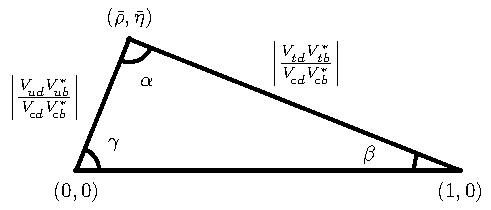
\includegraphics[scale=1]{diagram_ut}
      %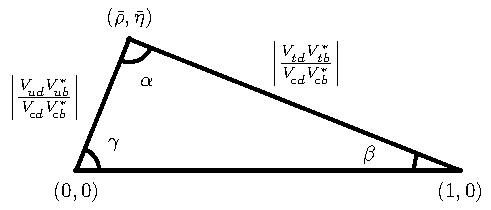
\includegraphics[width=0.48\textwidth]{diagram_ut}
      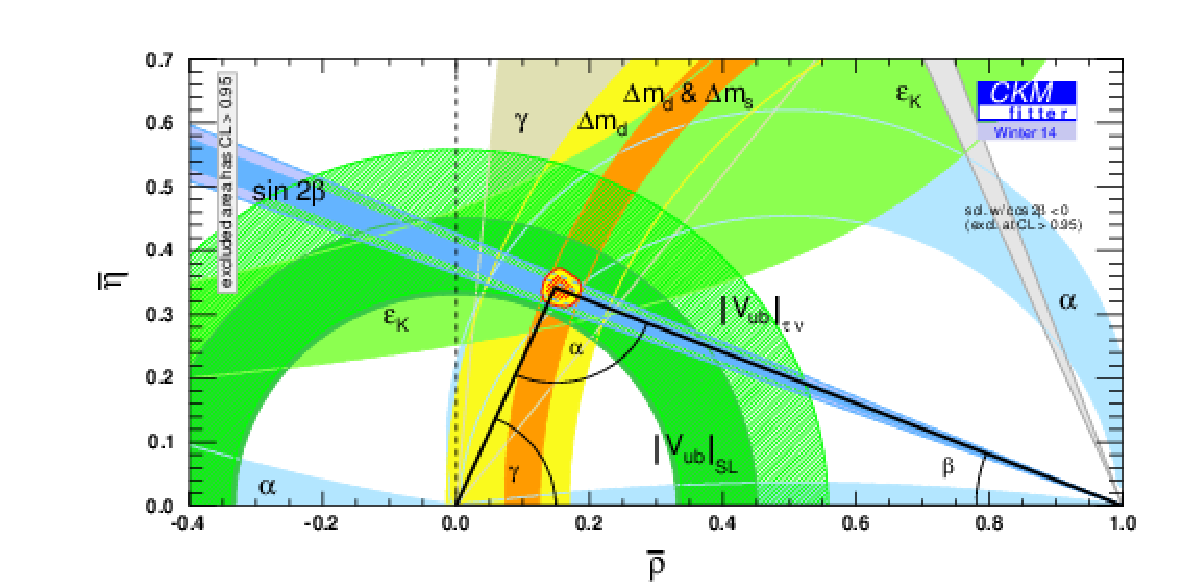
\includegraphics[width=0.47\textwidth]{rhoeta_small_Vub}
  \end{center}
  \caption[Unitarity triangle]{\small
    Schematic diagram of the Unitarity triangle given in Eq.~\ref{eq:th:ut} on the complex plane,
    where the base has been normalized to unit length.
    Alongside is shown the same triangle with coloured bands indicating various constraints on
    side lengths, angles and position of the apex.
  }
  \label{fig:th:ut}
\end{figure}

Precise determination of the CKM matrix elements is important, for  they are each fundamental
parameters of the SM.
They also contain all the information about flavour violation and CPV that is allowed within the
framework of the SM.
This information is reprtesented by the UT, a current fit of measurement of angles and side lengths
is shown in \Fig{fig:th:ut}.
If additional CP-violating phases were to exist beyond the SM, their effect would be seen in global
fits of the UT.

Each CKM matrix element is ususally measured in a particular way.
For example, the elements \V{td} and \V{ts} are measured using $B-\bar B$ oscillations since tree
level determination using \tquark quarks is difficult to do with precision.
However, the nature of NP is unknown and could effect different processes in different ways.
A good example of this is \V{ub}, which is the CKM element known to the lowest degree of accuracy.

A determination of \V{ub}
can be made using inclusive and exculsive measurements of
\decay{B}{X_u\ell\bar\nu_\ell} decays.
Inclusive measurements are made difficult from large
\decay{B}{X_c\ell\bar\nu_\ell} backgrounds, while exclusive semi-leptonic modes suffer from
uncertainties introduced by form factors.
A combination of these results leads to a value of
$\left|\V{ub}\right|_\mathrm{SL}=\left(4.13\pm0.49\right)\e{-3}$ \cite{PDG2012}.
But, \V{ub} can also be obtained using the tree level decay of
%A value of $\left|\V{ub}\right|$ can also be obtained from the annihilation decay
\decay{\Bp}{\taup\nu_\tau}:
$\left|\V{ub}\right|_{\tau\nu}=\left(4.22\pm0.42\right)\e{-3}$ \cite{PDG2012}.
The branching fraction which is used to calculate this latter value~\cite{Amhis:2012bh} is somewhat
higher than the SM prediction and particularly sensitive to NP models which include a charged
Higgs.
Figure \ref{fig:th:ut} shows the length of the side $|\V{ud}\Vconj{ub}|/|\V{cd}\Vconj{cb}|$
calculated by both values of \V{ub}.
The decay \btodsphi has a very similar topology to \decay{\Bp}{\taup\nu_\tau} in that it proceeds
via the annihilation of the \Bp meson constituent quarks and the resulting $W^+$ decays into quarks
that form the final state.
This decay is discussed in \Sec{sec:dsphi}.

The other side is sensitive to the value of \V{tb} and \V{td}.
The value of \V{tb} is determined from decays of \tquark quarks using the ratio
$\BF(\decay{t}{Wb})/\BF(\decay{t}{Wq})$, where $q=d,b,s$.
Oscillation frequencies of \Bd and \Bs mesons ($\Delta m_d$ and $\Delta m_s$ respectively) are used
to measure the \V{td} and \V{ts}.




\subsection{FCNCs}
Since the SM is such a good description of physics at energy scales that have been probed to date,
it is resonable to assume that this diverges at some cut off energy scale, $\Lambda$.
This scale can be set based on the solution of the hierarchy problem, which indicates that
$\Lambda$ should be less than a few TeV.
A bound can also be set on $\Lambda$ by considering processes which are absent from SM processes at
tree level, such as flavour changing neutral currnents (FCNCs).
This results in a value of $\Lambda$ which far exceeds the few TeV from solving the hierarchy
problem.
The conflict between these two determinations is named the \emph{Flavour Problem}.

The most pessimistic solution to the flavour problem is \emph{Minimal Flavour Violation} (MFV)
which simply assumes that beyond SM physics follows a Yukawa coupling like structure in the flavour
sector, this would lead to no discernable new physics in the flavour sector.


%The \decay{b}{s} FCNC is forbidden at tree level in the SM and are only allowed in higher-order
%electroweak processes.
%New particles from extensions to the SM can enter these loops and significantly alter




%Another indication of physics beyond the SM is that the Higgs mass ($\sim125\gev$) is close to the
%mass of the $W$ and $Z$ bosons.
%This means that loop level corrections.
%New physics contributing to these loops with the opposite sign to SM processes decrease the amount
%of fine tuning required.
%Particles entering into Higgs mass correction loops will enter in the same way into other loop
%processes.
%
%Particles from NP models con contribute


%As previously stated, there are no vertices exhibiting flavour changing neutral currents (FCNCs) in the SM.
%However, FCNCs can occur in loops diagrams.
%Because particles in these loops can be virtual, such processes have access to much higher mass
%scales than the energy supplied by the collision (by the Pauli exclusion principle).
%Therefore contributions from very massive particles can contribute...
%These particles will contribute to the amplitude of the overall interaction, such that loop level
%interactions...



%\section{The Flavour problem}
%It is natural to assume that the SM is only valid up to some energy scale $\Lambda$, where the
%value of the cut-off is undetermined.
%Using the argument of the hierarchy problem suggests that $\Lambda$ should be less than a few \tev.
%\bam{Motivates FCNCs}
%Beyond SM physics can be characterized by a general effective Lagrangian:
%\begin{equation}
  %\Lag{eff} = \sum_{n>2} \frac1{\Lambda^n}C_i\matho_i.
%\end{equation}
%Here, $\matho_i$ is an effective operator parameterizing the genera






%Therefore the
%Flavour changing neutral currents are forbidden, GIM...









%It is unknown how NP will manifest itself...
%
%
%
%Minimal Flavour Violation (MFV)
%
%
%FCNCs are forbidden...
%
%
%
%
%
%New particles...?
%Strong CP problem
%





%The Standard Model (SM) of particle physics explains interactions of fundamental particles and
%forces.
%It is a remarkably successful theory, which predicted the existence of a scalar Higgs boson which
%was discovered by the \cms and \atlas collaborations in 2012.
%The SM also predicts the value of the anomalous magnetic moment of the muon, $a_\mu$, which is in
%agreement with experimental results to five decimal places:
%\begin{align*}
  %%frac{g_\mu-2){2}
  %a_\mu^\mathrm{exp} &= \left(1165920.80 \pm 0.63\right)\e{-9} \\
  %a_\mu^\mathrm{th}  &= \left(1165918.41 \pm 0.48\right)\e{-9}.
%\end{align*}
%Despite these successes it is well known that the SM is incomplete, for it fails in several
%important points, for example: gravity is not included; neither dark matter, nor dark energy, is
%included; and neutrinos are treated as massless particles.
%Another problem is that the matter-antimatter asymmetry observable in the Universe cannot be
%reconciled by the SM.
%
%More than this example...
%%resolved



%This figure shows two, slightly conflicting, constraints for the side
%$|\V{ud}\Vconj{ub}|/|\V{cd}\Vconj{cb}|$ coming from different measurements of \V{ub}.
%One of these is from inclusive measurements of \decay{B}{X_u\ell\nu_\ell}, and the other is from
%This figure shows that the angle $\beta$ and
%\begin{figure}
  %\begin{center}
    %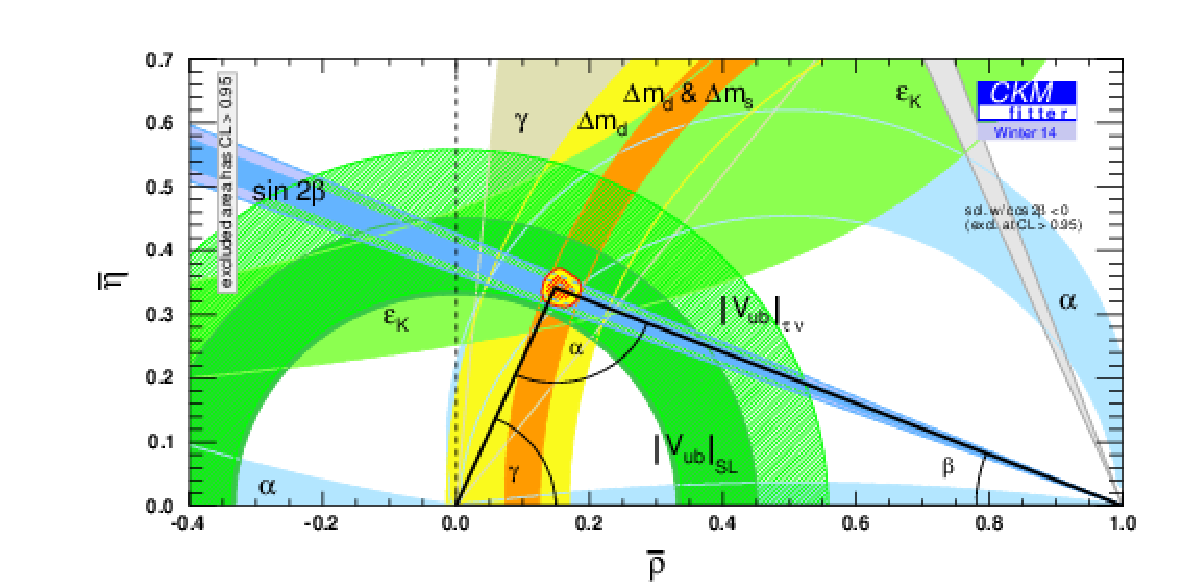
\includegraphics[width=0.5\textwidth]{rhoeta_small_Vub}
  %\end{center}
  %\caption[Unitary triangle measurements]{\small
    %Constraints on the UT in the complex plane. The $|\V{ub}|$ constraint is split into two
    %contributions: inclusive and exclusive semileptonic decays (plain dark green)
    %and $|\V{ub}|$ from \decay{\Bp}{\tau\nu_\tau} (hashed green).
    %The red hashed region of the global combination corresponds to 68\% CL.
  %}
  %\label{fig:th:ut2}
%\end{figure}

%One can write the Lagrangian

%\section{Testing the flavour sector of the SM}
%There are convincing/powerful/... reasons that

%If new physics were to enter as a CPV phase in the flavour sector of the SM, this would be seen in
%measurements of the angles and sides of the UT.
%The total particle physics Lagrangian can be written as:
%\begin{equation}
  %\Lag{Tot} = \Lag{SM} + \Lag{NP}.
%\end{equation}
%Additional CP-violating phases in \Lag{NP} would cause the triangle not to close, such that
%$\alpha+\beta+\gamma\neq\pi$.
%Therefore it is vital to measure the CKM matrix elements to as high a precision as possible in as
%many ways as possible.
%The current constraints on the UT are shown in Fig.~\ref{fig:th:ut2}.


%Diagonal elements of the CKM matrix are all known to high fractional precision...


%However, for all this, the SM fails to explain many phenomena:
%\begin{itemize}
  %\item There is no treatment for gravity.
  %\item There is no explanation for Dark Matter.
  %\item There is no explanation for Dark Energy.
  %\item Neutrinos are treated as massless.
  %\item Observed matter-antimatter asymmetry observable in the Universe.
%\end{itemize}

%There is no treatment
%\begin{itemize}
  %\item Quick overview of QED and QCD
  %\item All good, except for masses...
  %\item Then EWSB, new and full Lagrangian $B\vec{W} \to ZAW$
  %\item This parameterizes the behavior of all known particles to astounding accuracy
  %\item Masses are generated for $W, Z$ and not $\gamma$
  %\item Also get lepton \& quark masses
  %\item CKM matrix!
  %\item Wolfenstein parameterization
  %\item UT
  %\item CPV phase
  %\item Importance of measuring these parameters
  %\item Current status (CKM fitter/UTfit)
  %\item Trees and Loops
  %\item Incompleteness of SM - dark matter etc.
  %\item Also search for new physics directly (dark sector)
  %\item (Maybe MFV and why top quarks dominate in loops)
%\end{itemize}
%Done... All other theory can be handled in the specific analysis chapters.



%Spinor fields are (potentially) directly observable by experiment and obey the Dirac equation:
%\begin{equation}
  %(i\hbar\gamma^\mu\partial_\mu - mc)\psi = 0.
  %\label{th:eq:dirac}
%\end{equation}
%Therefore these particles, which are quanta of spinor fields, obey Fermi-Dirac statistics and are
%known as fermions.
%The fermions of the SM constitute six leptons (electron, muon, tauon and three corresponding
%neutrinos), and six quarks (up, down, charm, strange, top and bottom).
%Each fermion has an antiparticle with opposite charge (including neutrinos despite the fact they
%are neutral).
%Quanta of the vector and scalar fields obey Bose-Einstein staisitics and are the force carriers for
%the fundamental forces.
%These force mediators include the scalar Higgs boson, eight vector gluons of the string force and
%the vector $\gamma$, $W$ and $Z$ throught which the electroweak forces are mediated.
%
%
%Before SSB:
%This spontaneous symmetry breaking (SSB) of the $U(1)$ gauge symmetry directly  affects \Lag{Yuk}
%(Eq.~\ref{eq:th:lag}), which describes interactions between fermionic fields and the Higgs.
%It is not possible to dir...
%Before SSB the Yukawa coupling term for the quarks is:
%After this spontaneous symmetry breaking, the massive gauge bosons get a mass and the photon
%remains massless (as shown in Eq.~\ref{eq:th:lag}); it also affects \Lag{Yuk}.
%The Yukawa couplings describe the interactions of $\Phi$ with fermions:
%\begin{equation}
  %\Lag{Yuk} =
  %- \sum_{\substack{\ell= \\ e,\mu,\tau}}g_\ell\left(\bar\chi_L\Phi \ell_R + \bar \ell_R\Phi^\dagger\chi_L\right)
  %- y_{ij}^u\bar Q_L^i\Phi u_R^j
  %- y_{ij}^d\bar Q_L^i\tilde\Phi d_R^j + \mathrm{h.c.}.
%\end{equation}
%%Where $L$ and $R$ denote chiral fields,   % Define chiral fields earlier...
%Where $g_\ell$ and $y_{ij}^{u,d}$ are coupling constants and
%other terms are defined as:
%\begin{align}
  %\tilde\Phi_i &= \varepsilon_{ij}\Phi_j &
  %\chi_L &= \begin{pmatrix}\nu_L \\ \ell_L \end{pmatrix} &
  %Q_)L &= \begin{pmatrix}u_L \\ d_L \end{pmatrix}
%\end{align}
%for $u=u,c,t$ and $d=d,s,b$.
%After SSB and the Higgs potential acquires a VEV, \Lag{Yuk} can be split into an interaction term
%and a mass term, where the interaction term defines couplings between fermions and the Higgs
%($H\bar\psi\psi$), and the mass term is:
%\begin{equation}
  %\Lag{Yuk,mass} =
  %-\sum_{\ell=e,\mu,\tau}g_\ell\frac{v}{\sqrt{2}}
  %\left(\bar\ell_R\ell_L + \bar\ell_L\ell_R\right)
  %-\frac{v}{\sqrt{2}} y_{ij}^u\bar u_L^iu_{R,j}
  %-\frac{v}{\sqrt{2}} y_{ij}^d\bar d_L^id_{R,j},
  %%\mathrm{so} m_{u,d} = \frac{v}{\sqrt{2}}y_{ij}^{u,d}.
%\end{equation}
%and the mass of the quarks is given by the mass matrix
%$m^{u,d}_{ij} = \frac{v}{\sqrt{2}}y_{ij}^{u,d}$.
%This matrix can be diagonalized such that $m_{ij}^\mathrm{diag} = V_{Lik}m_{kl}(V_R^\dagger)_{lj}$
%which equates to rotating the left- and right-handed chiral quark fields with the matrices
%$V_L$ and $V_R$, respectively.
%Rotating the basis of quarks does not affect any of the mass or Higgs coupling terms of the quarks,
%but does change \Lag{q}:
%\begin{align}
  %\Lag{q}
  %&= \frac{g}{2}i\gamma^\mu
  %\left[\bar u_Ld_LW^+_\mu + \bar d_Lu_LW^-_\mu
  %\right] + \Lag{q}^\mathrm{NC} + \Lag{q}^\gamma \\
  %&\to \frac{g}{2}i\gamma^\mu
  %\left[
    %\bar u_L\left(V_{uL}V_{dL}^\dagger\right)d_LW^+_\mu +
    %\bar d_L\left(V_{dL}V_{uL}^\dagger\right)u_LW^-_\mu
  %\right] + \Lag{q}^\mathrm{NC} + \Lag{q}^\gamma.
%\end{align}
%Where $\Lag{q}^\mathrm{NC}$ and $\Lag{q}^\gamma$ are the weak neutral current and photon currents
%for quarks.
%These also remain invariant under the basis change, for example:
%\begin{align}
  %\Lag{NC}
  %&= i\sqrt{g^2+g^{\prime2}}
  %\left(
  %Z_\mu\bar u_j \gamma^\mu\left(g_v-\gamma_5g_A\right)u_j +
  %Z_\mu\bar d_j \gamma^\mu\left(g_v-\gamma_5g_A\right)d_j
  %\right)
  %\\
  %&\to i\sqrt{g^2+g^{\prime2}}
  %\left(
  %Z_\mu\bar u_j \gamma^\mu\left(g_v-\gamma_5g_A\right)\left(VV\right)u_j +
  %Z_\mu\bar d_j \gamma^\mu\left(g_v-\gamma_5g_A\right)\left(VV\right)d_j
  %\right)
  %\label{eq:th:nc}
%\end{align}
%where $VV=\mathbb{1}$ by unitarity.
%The matrix $V = \left(V_{uL}V_{dL}^\dagger\right)$ parameterizes the couplings between up- and
%down-type quarks in charged weak currents and is known as the Cabibbo-Kobayashi-Maskawa (CKM)
%matrix.
